\chapter{طراحی جاذب های دینامیکی ارتعاش به وسیله بهینه سازی الگوریتم ژنتیک}
\section{مقدمه}

بهینه‌سازی مرسوم \lr{DVA} کنترل مستقیم اندکی بر شکل‌دهی پاسخ فرکانسی (\lr{FRF}) فراهم می‌کند و به علت ضعف در غربالگری پارامترها، متغیرهای غیرضروری در مدل باقی می‌مانند. این موضوع منجر به طرح‌هایی بیش‌پارامتری و پیچیده می‌شود. در این پژوهش، یک معیار یکتا با نام \(C_s\) معرفی شده است که اهداف نرمال‌شده و وزن‌دار مرتبط با موقعیت قله‌ها، دامنه قله‌ها، پهنای‌باند و سایر عوامل را در یک چارچوب یکپارچه ترکیب می‌کند. افزون بر این، یک ترم خاصِ تنک‌سازی در تابع هدف لحاظ شده است که مانع از ورود پارامترهای زائد و غیرضروری می‌گردد. 

چارچوب پیشنهادی در نرم‌افزار \lr{DeVana} که توسط نویسندگان توسعه یافته است پیاده‌سازی شده و برای یک بنچمارک \lr{1DOF–1DOF} کاملاً کوپل‌شده مورد استفاده قرار گرفته است. این مطالعه موردی شامل یک باند اجتناب مشخص در بازه فرکانسی \lr{1000–2000 Hz} می‌باشد. 

نتایج نشان داد که \lr{DVA} بهینه‌شده رزونانس پایه را به دو قله باریک در لبه‌های باند تقسیم کرده و پاسخ درون‌باندی را تضعیف می‌کند، در حالی که بخش عمده‌ای از پارامترهای \(\nu\) به سمت صفر همگرا می‌شوند و تنها مجموعه محدودی از پارامترهای \(\beta\)، \(\lambda\) و \(\mu\) فعال باقی می‌مانند. فرآیند بهینه‌سازی در مقدار بهینه برازندگی \(\,0.001206\) همگرا شد. 

سهم اجزای تابع هدف در این مقدار بهینه به‌ترتیب شامل $40.8\%$ از معیار \(C_s\)، برابر با $34.7\%$ از جریمه تنک‌سازی و $24.5\%$ از ترم دقت هدف‌گیری است. 

به‌طور کلی، تجمیع اهداف طراحی در قالب یک تابع هدف تفسیرپذیر واحد، امکان هدف‌گذاری مستقیم \lr{FRF} و سنتز ساده‌شده \lr{DVA} را فراهم می‌سازد. این رویکرد منجر به تنظیم سریع و منطبق با معیارها می‌شود، در حالی که تنها حداقل مجموعه‌ای از پارامترهای غربال‌شده در طراحی باقی می‌ماند.

\section{بيان مسئله}

\subsection{تعريف سيستم مكانيكي}

\subsubsection{ سيستم كاملاً كوپل‌شده \lr{2DOF - 3DOF}}
\paragraph{مرور كلي سيستم و پيكربندي}

براي درك مفاهيم پايه و اصول عملياتي روش الگوريتم ژنتيك پيشرفته‌اي كه در اين كار معرفي شده است، يك تحليل جامع و گام‌به‌گام از سيستم مكانيكي ضروري است. سيستم مورد بررسي يك سيستم پيشرفته كاملاً كوپل‌شده \lr{2DOF - 3DOF} است؛ منظور از «كاملاً كوپل‌شده» آن است كه تمام اجزاي سيستم از طريق جرم‌ها، فنرها، دمپرها و \lr{inerter}‌ها به يكديگر متصل شده‌اند و يك سيستم ارتعاشي كامل با برهم‌كنش‌هاي ديناميكي فراگير را تشكيل مي‌دهند. شماتیکی از این سیستم در شکل 
\ref{fig:2DOF-3DOF schematic}
نمایش داده شده است. 

\begin{figure}
  \centering
  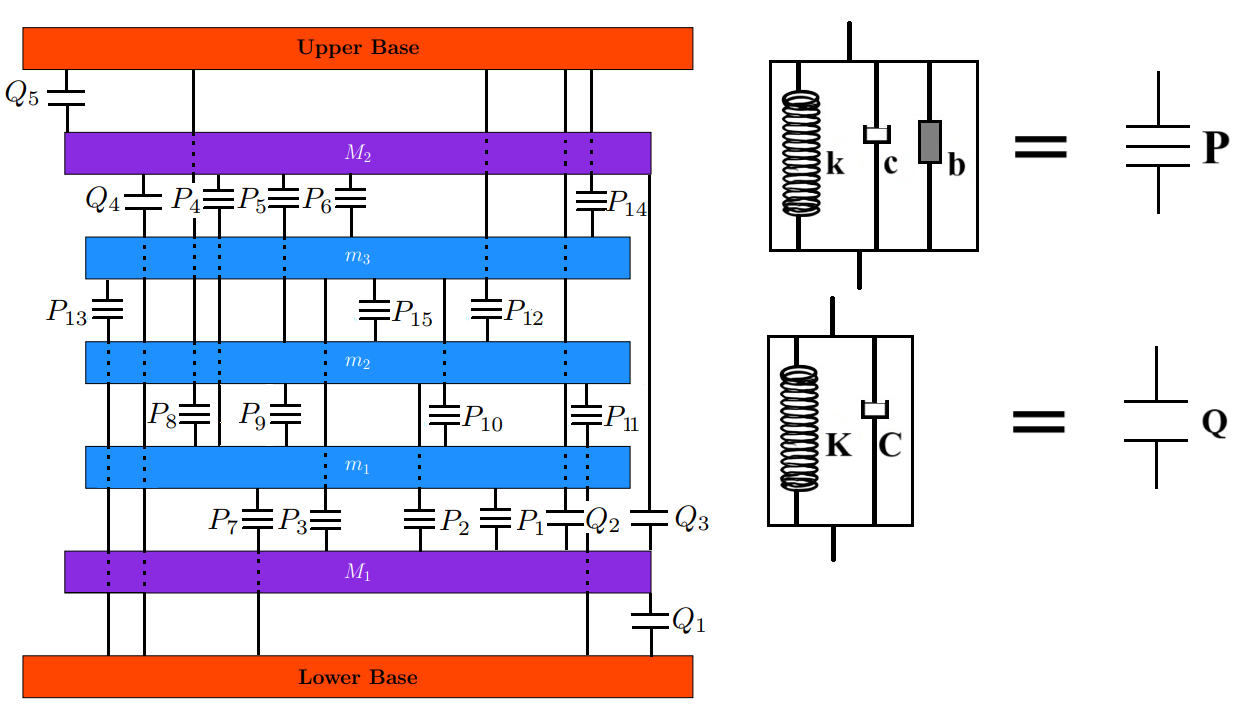
\includegraphics[width=\textwidth]{picture10.png}
  \caption{شماتیکی از سیستم کاملا کوپل شده \lr{2DOF-3DOF}}\label{fig:2DOF-3DOF schematic}
\end{figure}


ساختار اصلي از يك سيستم اصلي دو درجه آزادی با دو جرم اصلي كه نمايانگر اجزاي متفاوت سازه هستند تشكيل شده و با سه جاذب‌ ارتعاشات ديناميكي \lr{DVA} تك‌درجه آزادي كه به‌طور راهبردي در موقعيت‌هاي مناسب قرار گرفته‌اند، تقويت شده است. اين پيكربندي امكان كنترل ارتعاش چند-مودي را فراهم مي‌كند و به صورت همزمان چندين فركانس رزونانس را هدف مي‌گيرد. معماري سيستم شامل موارد زير است:

\begin{itemize}
    \item \textbf{اجزاي سازه‌اي اصلي}: دو جرم اصلي ($M_1$, $M_2$) كه اجزاي اصلي سازه را با خواص اينرسي‌شان نمايش مي‌دهند
    \item \textbf{جذب‌كننده‌هاي ارتعاش ديناميكي}: سه جرم \lr{DVA} ($\mu_1$, $\mu_2$, $\mu_3$) با ويژگي‌هاي ديناميكي مستقل
    \item \textbf{تحريك‌هاي پايه}: حركات پايه پاييني و بالايي كه ورودي‌هاي ارتعاشي خارجي را فراهم مي‌كنند
    \item \textbf{نياور خارجي}: اعمال مستقيم نيروي خارجي بر جرم‌هاي اصلي
    \item \textbf{كوپلينگ كامل}: درهم‌پيوستگي همه اجزا از طريق مؤلفه‌هاي جرمي، سختي، دمپينگ و اينرسي
\end{itemize}

پيچيدگي سيستم از فضاي پارامتري گسترده و سازوكارهاي كوپلينگ ناشي مي‌شود. كل سيستم از 48 پارامتر طراحي مستقل تشكيل شده است كه در ميان گروه‌هاي زير توزيع شده‌اند:
\begin{itemize}
    \item 15 پارامتر كوپلينگ جرمي ($\beta_1$ تا $\beta_{15}$) براي اتصالات اينرسي
    \item 15 پارامتر سختي ($\lambda_1$ تا $\lambda_{15}$) براي كوپلينگ الاستيك
    \item 15 پارامتر دمپينگ ($\nu_1$ تا $\nu_{15}$) براي اتلاف انرژي
    \item 3 پارامتر جرم \lr{DVA} ($\mu_1$, $\mu_2$, $\mu_3$) براي تعيين اندازه جذب‌كننده‌ها
\end{itemize}

اين فضاي پارامتري پُربعد نيازمند به‌كارگيري تكنيك‌هاي بهينه‌سازي پيشرفته‌اي است كه بتوانند دامنه طراحي را به‌صورت كارآمد جستجو كنند و در عين حال قابليت محاسباتي را حفظ نمايند.

\paragraph{مدل‌سازي ارتعاشي سيستم و فرضيات}

سيستم اصلي \lr{2DOF} با استفاده از چارچوبي جامع شامل جرم‌ها، فنرها، دمپرها و \lr{inerter}‌ها و با اتصال به هر دو پايه بالا و پايه پايين مدل‌سازي مي‌شود. رويكرد مدل‌سازي بر فرضيات بنيادي زير استوار است:

\begin{itemize}
    \item \textbf{رفتار الاستيك خطي}: تمام مؤلفه‌هاي سختي ($K_1$, $K_2$, $K_3$) در بازه عملياتي از رابطه نيرو–جابجايي خطي پيروي مي‌كنند
    \item \textbf{دمپينگ ويسكوز خطي}: تمام مؤلفه‌هاي دمپينگ ($C_1$, $C_2$, $C_3$) از روابط نيروي وابسته به سرعت خطي تبعيت مي‌كنند
    \item \textbf{نمايش جرم نقطه‌اي}: تمام جرم‌ها به‌صورت جرم نقطه‌اي با خواص اينرسي متمركز در نظر گرفته مي‌شوند
    \item \textbf{حركت يك‌بعدي}: تمام مؤلفه‌هاي سيستم تنها در يك راستاي انتقالی حركت مي‌كنند
    \item \textbf{پارامترهاي ثابت در زمان}: همه پارامترهاي سيستم در طول بهره‌برداري ثابت هستند
    \item \textbf{عدم وجود غيرخطيي هندسي}: سيستم در ناحيه خطي عمل مي‌كند و اثرات سفت‌شدگي هندسي ناديده گرفته مي‌شود
    \item \textbf{اتصال كامل و صلب}: همه درگاه‌ها و اتصالات بين اجزا به‌صورت صلب و كامل فرض مي‌شوند
\end{itemize}

تحريك‌هاي پايه با انعطاف‌پذيري به‌گونه‌اي مدل‌سازي مي‌شوند كه سناريوهاي گوناگون مكانيكي را بازنمايي كنند:
\begin{itemize}
    \item \textbf{حركت فونداسيون}: نمايانگر حركت واقعي زمين يا تحريك تكيه‌گاه
    \item \textbf{مودهاي اضافي سيستم}: مدل‌سازي درجات آزادي اضافي ناشي از سازه‌هاي پيچيده‌تر
    \item \textbf{تغييرات شرايط مرزي}: سازگاري با شرايط گوناگون تكيه‌گاه و نصب
\end{itemize}

هر \lr{DVA} به‌صورت مستقل به شكل يك سيستم تك‌درجه آزادي با جرم، سختي، دمپينگ و مؤلفه‌هاي اينرسي اختصاصي خود طراحي شده است. كوپلينگ ميان سيستم اصلي و \lr{DVA}‌ها و نيز ميان خود \lr{DVA}‌ها از طريق مؤلفه‌هاي اتصال جامع انجام مي‌شود تا كوپلينگ ديناميكي كامل تضمين گردد.

\paragraph{استخراج معادلات حاكم}

معادلات حاكم براي سيستم كاملاً كوپل‌شده \lr{2DOF-3DOF} با استفاده از روش \lr{Newton} و با اعمال قانون دوم \lr{Newton} بر هر درجه آزادي و در نظر گرفتن تمام نيروهاي اتصال‌دهنده استخراج مي‌شوند. مختصات تعميم‌يافته سيستم به صورت زير تعريف مي‌گردند:

\begin{align}\label{Eq.generalized.coordinate.2dof3dof}
    \mathbf{q} =
    \begin{bmatrix}
        U_1(t) \\
        U_2(t) \\
        u_1(t) \\
        u_2(t) \\
        u_3(t)
    \end{bmatrix}; \quad
    \dot{\mathbf{q}} =
    \begin{bmatrix}
        \dot{U_1}(t) \\
        \dot{U_2}(t) \\
        \dot{u_1}(t) \\
        \dot{u_2}(t) \\
        \dot{u_3}(t)
    \end{bmatrix}; \quad
    \ddot{\mathbf{q}} =
    \begin{bmatrix}
        \ddot{U_1}(t) \\
        \ddot{U_2}(t) \\
        \ddot{u_1}(t) \\
        \ddot{u_2}(t) \\
        \ddot{u_3}(t)
    \end{bmatrix}
\end{align}

كه در آن:
\begin{itemize}
    \item $U_1(t)$، $U_2(t)$: جابجايي‌هاي جرم‌هاي اصلي در زمان $t$
    \item $u_1(t)$، $u_2(t)$، $u_3(t)$: جابجايي‌هاي جرم‌هاي \lr{DVA} در زمان $t$
\end{itemize}

معادلات حركت به صورت ماتريسي بيان مي‌شوند:

\begin{equation} \label{Eq.EOM_dimensional_combined}
    \mathbf{M} \ddot{\mathbf{q}} + \mathbf{C} \dot{\mathbf{q}} + \mathbf{K} \mathbf{q} = \mathbf{F}(t)
\end{equation}

كه در آن:

\begin{itemize}
    \item $\mathbf{q}$: بردار جابجايي‌هاي تعميم‌يافته كه جابجايي جرم‌هاي اصلي و جرم‌هاي \lr{DVA} را دربر مي‌گيرد.
    \item $\mathbf{M}$: ماتريس جرم.
    \item $\mathbf{C}$: ماتريس دمپينگ.
    \item $\mathbf{K}$: ماتريس سختي.
    \item $\mathbf{F}(t)$: بردار نيروي خارجي كه هم بارهاي خارجي و هم آثار حركت پايه را شامل مي‌شود.
\end{itemize}

بردار مختصات تعميم‌يافته به صورت زير بازتعريف مي‌شود:

\begin{equation}\label{Eq.generalized_coordinate_combined}
    \mathbf{q} = 
  \begin{bmatrix}
    U_1 \\ U_2 \\ u_1 \\ u_2 \\ u_3
  \end{bmatrix}
\end{equation}

\paragraph{ماتريس جرم}

\begin{equation}\label{Eq.mass_matrix_dimensional_combined}
\begin{aligned}
[M] =& 
\begin{bmatrix}
\shortstack[c]{$M_1 + b_1$ \\ $+ b_2 + b_3$} & 0 & \shortstack[c]{$-b_1$ \\ \,} & \shortstack[c]{$-b_2$ \\ \,} & \shortstack[c]{$-b_3$ \\ \,} \\
0 & \shortstack[c]{$M_2 + b_4$ \\ $+ b_5 + b_6$} & \shortstack[c]{$-b_4$ \\ \,} & \shortstack[c]{$-b_5$ \\ \,} & \shortstack[c]{$-b_6$ \\ \,} \\
\shortstack[c]{$-b_1$ \\ \,} & \shortstack[c]{$-b_4$ \\ \,} & \shortstack[c]{$m_1 + b_1$ \\ $+ b_4 + b_7$ \\ $+ b_8 + b_9$ \\ $+ b_{10}$} & \shortstack[c]{$-b_9$ \\ \,} & \shortstack[c]{$-b_{10}$ \\ \,} \\
\shortstack[c]{$-b_2$ \\ \,} & \shortstack[c]{$-b_5$ \\ \,} & \shortstack[c]{$-b_9$ \\ \,} & \shortstack[c]{$m_2 + b_2$ \\ $+ b_5 + b_9$ \\ $+ b_{11} + b_{12}$} & \shortstack[c]{$-b_{15}$ \\ \,} \\
\shortstack[c]{$-b_3$ \\ \,} & \shortstack[c]{$-b_6$ \\ \,} & \shortstack[c]{$-b_{10}$ \\ \,} & \shortstack[c]{$-b_{15}$ \\ \,} & \shortstack[c]{$m_3 + b_3$ \\ $+ b_6 + b_{10}$ \\ $+ b_{13} + b_{14}$ \\ $+ b_{15}$}
\end{bmatrix}
\end{aligned}
\end{equation}

\paragraph{ماتريس دمپينگ}

\begin{equation}\label{Eq.damping_matrix_dimensional_combined}
\begin{aligned}
[C] =& 
\begin{bmatrix}
\shortstack{$C_1 + C_2$ \\ $+ C_3$} & -C_3 & \shortstack{$-c_1$ \\ \,} & \shortstack{$-c_2$ \\ \,} & \shortstack{$-c_3$ \\ \,} \\
-C_3 & \shortstack{$C_3 + C_4$ \\ $+ C_5 + c_4$ \\ $+ c_5 + c_6$} & \shortstack{$-c_4$ \\ \,} & \shortstack{$-c_5$ \\ \,} & \shortstack{$-c_6$ \\ \,} \\
-c_1 & -c_2 & \shortstack{$c_1 + c_4$ \\ $+ c_7 + c_8$ \\ $+ c_9 + c_{10}$} & \shortstack{$-c_9$ \\ \,} & \shortstack{$-c_{10}$ \\ \,} \\
-c_2 & -c_5 & -c_9 & \shortstack{$c_2 + c_5$ \\ $+ c_9 + c_{11}$ \\ $+ c_{12} + c_{15}$} & \shortstack{$-c_{15}$ \\ \,} \\
-c_3 & -c_{6} & -c_{10} & -c_{15} & \shortstack{$c_3 + c_6$ \\ $+ c_{10} + c_{13}$ \\ $+ c_{14} + c_{15}$}
\end{bmatrix}
\end{aligned}
\end{equation}

\paragraph{ماتريس سختي}

\begin{equation}\label{Eq.stiffness_matrix_dimensional_combined}
\begin{aligned}
[K] =& 
\begin{bmatrix}
\shortstack{$K_1 + K_2$ \\ $+ K_3$} & -K_3 & \shortstack{$-k_1$ \\ \,} & \shortstack{$-k_2$ \\ \,} & \shortstack{$-k_3$ \\ \,} \\
-K_3 & \shortstack{$K_3 + K_4$ \\ $+ K_5 + k_4$ \\ $+ k_5 + k_6$} & \shortstack{$-k_4$ \\ \,} & \shortstack{$-k_5$ \\ \,} & \shortstack{$-k_6$ \\ \,} \\
-k_1 & -k_2 & \shortstack{$k_1 + k_4$ \\ $+ k_7 + k_8$ \\ $+ k_9 + k_{10}$} & \shortstack{$-k_9$ \\ \,} & \shortstack{$-k_{10}$ \\ \,} \\
-k_2 & -k_5 & -k_9 & \shortstack{$k_2 + k_5$ \\ $+ k_9 + k_{11}$ \\ $+ k_{12} + k_{15}$} & \shortstack{$-k_{15}$ \\ \,} \\
-k_3 & -k_{6} & -k_{10} & -k_{15} & \shortstack{$k_3 + k_6$ \\ $+ k_{10} + k_{13}$ \\ $+ k_{14} + k_{15}$}
\end{bmatrix}
\end{aligned}
\end{equation}

\paragraph{بردار نيرو}

\begin{equation}\label{Eq.force_vector_dimensional_combined}
\begin{aligned}
[F] = & \begin{bmatrix}
F_1(t) + C_1 \dot{U}_{low} + C_2 \dot{U}_{upp} + K_1 U_{low} + K_2 U_{upp} \\
F_2(t) + C_4 \dot{U}_{low} + C_5 \dot{U}_{upp} + K_4 U_{low} + K_5 U_{upp} \\
\beta_7 \ddot{U}_{low} + \beta_8 \ddot{U}_{upp} + 2 \zeta_{dc} \omega_{dc} (\nu_7 \dot{U}_{low} + \nu_8 \dot{U}_{upp}) + \omega_{dc}^2 (\lambda_7 U_{low} + \lambda_8 U_{upp}) \\
\beta_{11} \ddot{U}_{low} + \beta_{12} \ddot{U}_{upp} + 2 \zeta_{dc} \omega_{dc} (\nu_{11} \dot{U}_{low} + \nu_{12} \dot{U}_{upp}) + \omega_{dc}^2 (\lambda_{11} U_{low} + \lambda_{12} U_{upp}) \\
\beta_{13} \ddot{U}_{low} + \beta_{14} \ddot{U}_{upp} + 2 \zeta_{dc} \omega_{dc} (\nu_{13} \dot{U}_{low} + \nu_{14} \dot{U}_{upp}) + \omega_{dc}^2 (\lambda_{13} U_{low} + \lambda_{14} U_{upp})
\end{bmatrix}
\end{aligned}
\end{equation}

\subsubsection{صورت بي‌بعد}

به‌منظور ساده‌سازي تحليل، سيستم با استفاده از پارامترهاي بي‌بعدِ فهرست‌شده در جدول~\ref{Tab:dimensionless.table} نرمال‌سازي مي‌شود.

\begin{table}[h!]
\centering
\caption{پارامترهاي بي‌بعد براي نرمال‌سازي سيستم}
\label{Tab:dimensionless.table}
\begin{tabular}{lcc}
\toprule
\textbf{گروه پارامتر} & \textbf{پارامتر} & \textbf{تعريف} \\
\midrule
\textbf{نسبت‌هاي جرم} & \( \Gamma \) & \( \Gamma = \frac{M_2}{M_1} \) \\
 & \( \mu_i \) & \( \mu_i = \frac{m_i}{M_1} \) \\
\addlinespace
\textbf{نسبت‌هاي كوپلينگ اينرسي} & \( \beta_i \) & \( \beta_i = \frac{b_i}{M_1} \) \\
\addlinespace
\textbf{نسبت‌هاي دمپينگ} & \( \mathcal{N}_i \) & \( \mathcal{N}_i = \frac{C_i}{C_1} \) \\
 & \( \nu_i \) & \( \nu_i = \frac{c_i}{C_1} \) \\
\addlinespace
\textbf{نسبت‌هاي سختي} & \( \Lambda_i \) & \( \Lambda_i = \frac{K_i}{K_1} \) \\
 & \( \lambda_i \) & \( \lambda_i = \frac{k_i}{K_1} \) \\
\addlinespace
\textbf{سيستم اصليِ بدون كوپل} & \( \omega_{dc} \) & \( \omega_{dc} = \sqrt{\frac{K_1}{M_1}} \) \\
 & \( \zeta_{dc} \) & \( \zeta_{dc} = \frac{C_1}{2 M_1 \omega_{dc}} \) \\
\bottomrule
\end{tabular}
\end{table}

با استفاده از اين پارامترها، معادلات بي‌بعد حركت به صورت زير بيان مي‌شوند:

\begin{equation}\label{Eq.EOM_dimensionless}
\mathbf{\bar{M}} \ddot{\mathbf{q}} + 2 \zeta_{dc} \omega_{dc} \mathbf{\bar{C}} \dot{\mathbf{q}} + \omega_{dc}^2 \mathbf{\bar{K}} \mathbf{q} = \mathbf{\bar{F}}(t)
\end{equation}

ماتريس‌هاي بي‌بعد جرم، دمپينگ و سختي به همراه بردار نيرو در روابط \eqref{Eq.mass_matrix_dimensionless} تا \eqref{Eq.force_vector_dimensionless} تعريف مي‌شوند.

\paragraph{ماتريس جرمِ بي‌بعد}

\begin{equation}\label{Eq.mass_matrix_dimensionless}
\begin{aligned}
[\bar{M}] =& 
\begin{bmatrix}
\shortstack{$1 + \beta_1$ \\ $+ \beta_2 + \beta_3$} & 0 & \shortstack{$-\beta_1$ \\ \,} & \shortstack{$-\beta_2$ \\ \,} & \shortstack{$-\beta_3$ \\ \,} \\
0 & \shortstack{$\Gamma + \beta_4$ \\ $+ \beta_5 + \beta_6$} & \shortstack{$-\beta_4$ \\ \,} & \shortstack{$-\beta_5$ \\ \,} & \shortstack{$-\beta_6$ \\ \,} \\
-\beta_1 & -\beta_4 & \shortstack{$\mu_1 + \beta_1$ \\ $+ \beta_4 + \beta_7$ \\ $+ \beta_8 + \beta_9$ \\ $+ \beta_{10}$} & \shortstack{$-\beta_9$ \\ \,} & \shortstack{$-\beta_{10}$ \\ \,} \\
-\beta_2 & -\beta_5 & -\beta_9 & \shortstack{$\mu_2 + \beta_2$ \\ $+ \beta_5 + \beta_9$ \\ $+ \beta_{11} + \beta_{12}$} & \shortstack{$-\beta_{15}$ \\ \,} \\
-\beta_3 & -\beta_6 & -\beta_{10} & -\beta_{15} & \shortstack{$\mu_3 + \beta_3$ \\ $+ \beta_6 + \beta_{10}$ \\ $+ \beta_{13} + \beta_{14}$ \\ $+ \beta_{15}$}
\end{bmatrix}
\end{aligned}
\end{equation}

\paragraph{ماتريس دمپينگِ بي‌بعد}

\begin{equation}\label{Eq.damping_matrix_dimensionless}
\begin{aligned}
[\bar{C}] =& 
\begin{bmatrix}
\shortstack{$1 + \mathcal{N}_2$ \\ $+ \mathcal{N}_3 + \nu_1$ \\ $+ \nu_2 + \nu_3$} & -\mathcal{N}_3 & \shortstack{$-\nu_1$ \\ \,} & \shortstack{$-\nu_2$ \\ \,} & \shortstack{$-\nu_3$ \\ \,} \\
-\mathcal{N}_3 & \shortstack{$\mathcal{N}_3 + \mathcal{N}_4$ \\ $+ \mathcal{N}_5 + \nu_4$ \\ $+ \nu_5 + \nu_6$} & \shortstack{$-\nu_4$ \\ \,} & \shortstack{$-\nu_5$ \\ \,} & \shortstack{$-\nu_6$ \\ \,} \\
-\nu_1 & -\nu_2 & \shortstack{$\nu_1 + \nu_4$ \\ $+ \nu_7 + \nu_8$ \\ $+ \nu_9 + \nu_{10}$} & \shortstack{$-\nu_9$ \\ \,} & \shortstack{$-\nu_{10}$ \\ \,} \\
-\nu_2 & -\nu_5 & -\nu_9 & \shortstack{$\nu_2 + \nu_5$ \\ $+ \nu_9 + \nu_{11}$ \\ $+ \nu_{12} + \nu_{15}$} & \shortstack{$-\nu_{15}$ \\ \,} \\
-\nu_3 & -\nu_{6} & -\nu_{10} & -\nu_{15} & \shortstack{$\nu_3 + \nu_6$ \\ $+ \nu_{10} + \nu_{13}$ \\ $+ \nu_{14} + \nu_{15}$}
\end{bmatrix}
\end{aligned}
\end{equation}

\paragraph{ماتريس سختيِ بي‌بعد}

\begin{equation}\label{Eq.stiffness_matrix_dimensionless}
\begin{aligned}
[\bar{K}] =& 
\begin{bmatrix}
\shortstack{$1 + \Lambda_2$ \\ $+ \Lambda_3 + \lambda_1$ \\ $+ \lambda_2 + \lambda_3$} & -\Lambda_3 & \shortstack{$-\lambda_1$ \\ \,} & \shortstack{$-\lambda_2$ \\ \,} & \shortstack{$-\lambda_3$ \\ \,} \\
-\Lambda_3 & \shortstack{$\Lambda_3 + \Lambda_4$ \\ $+ \Lambda_5 + \lambda_4$ \\ $+ \lambda_5 + \lambda_6$} & \shortstack{$-\lambda_4$ \\ \,} & \shortstack{$-\lambda_5$ \\ \,} & \shortstack{$-\lambda_6$ \\ \,} \\
-\lambda_1 & -\lambda_2 & \shortstack{$\lambda_1 + \lambda_4$ \\ $+ \lambda_7 + \lambda_8$ \\ $+ \lambda_9 + \lambda_{10}$} & \shortstack{$-\lambda_9$ \\ \,} & \shortstack{$-\lambda_{10}$ \\ \,} \\
-\lambda_2 & -\lambda_5 & -\lambda_9 & \shortstack{$\lambda_2 + \lambda_5$ \\ $+ \lambda_9 + \lambda_{11}$ \\ $+ \lambda_{12} + \lambda_{15}$} & \shortstack{$-\lambda_{15}$ \\ \,} \\
-\lambda_3 & -\lambda_{6} & -\lambda_{10} & -\lambda_{15} & \shortstack{$\lambda_3 + \lambda_6$ \\ $+ \lambda_{10} + \lambda_{13}$ \\ $+ \lambda_{14} + \lambda_{15}$}
\end{bmatrix}
\end{aligned}
\end{equation}

\paragraph{بردار نيروي بي‌بعد}

\begin{equation}\label{Eq.force_vector_dimensionless}
\begin{aligned}
[\bar{F}] = & \begin{bmatrix}
\frac{F_1(t)}{M_1} + 2 \zeta_{dc} \omega_{dc} (\dot{U}_{low} + \mathcal{N}_2 \dot{U}_{upp}) + \omega_{dc}^2 (U_{low} + \Lambda_2 U_{upp})\\
\frac{F_2(t)}{M_1} + 2 \zeta_{dc} \omega_{dc} (\mathcal{N}_4 \dot{U}_{low} + \mathcal{N}_5 \dot{U}_{upp}) + \omega_{dc}^2 (\Lambda_4 U_{low} + \Lambda_5 U_{upp}) \\
\beta_7 \ddot{U}_{low} +  \beta_8 \ddot{U}_{upp} +  2 \zeta_{dc} \omega_{dc} (\nu_7 \dot{U}_{low} + \nu_8 \dot{U}_{upp}) +\omega_{dc}^2 (\lambda_7 U_{low} + \lambda_8 U_{upp})\\
\beta_{11} \ddot{U}_{low} +  \beta_{12} \ddot{U}_{upp} +  2 \zeta_{dc} \omega_{dc} (\nu_{11} \dot{U}_{low} + \nu_{12} \dot{U}_{upp}) +\omega_{dc}^2 (\lambda_{11} U_{low} + \lambda_{12} U_{upp})\\
\beta_{13} \ddot{U}_{low} +  \beta_{14} \ddot{U}_{upp} +  2 \zeta_{dc} \omega_{dc} (\nu_{13} \dot{U}_{low} + \nu_{14} \dot{U}_{upp}) +\omega_{dc}^2 (\lambda_{13} U_{low} + \lambda_{14} U_{upp})
\end{bmatrix}
\end{aligned}
\end{equation}

\paragraph{راه‌حل‌هاي نيم تحليلي براي تحريك هارمونيك}

روش نيم تحليلي بر تحريك هارمونيك و حركت هم‌فاز تكيه دارد. پاسخ سيستم به صورت زير بيان مي‌شود:

\begin{align}\label{Eq.harmonic.solution.2dof3dof}
    \begin{bmatrix}
        U_1(t) \\
        U_2(t) \\
        u_1(t) \\
        u_2(t) \\
        u_3(t)
    \end{bmatrix} =
    \begin{bmatrix}
        A_1 \\
        A_2 \\
        a_1 \\
        a_2 \\
        a_3
    \end{bmatrix} e^{j \omega t}
\end{align}

كه در آن $A_1, A_2$ دامنه ارتعاش جرم‌هاي اصلي و $a_1, a_2, a_3$ دامنه ارتعاش جرم‌هاي \lr{DVA} هستند.

تحريك‌هاي هارمونيك به صورت زير تعريف مي‌شوند:

\begin{align}\label{Eq.harmonic.excitations.2dof3dof}
    \begin{split}
        F_1(t) &= F_1 e^{j \omega t} \\
        F_2(t) &= F_2 e^{j \omega t} \\
        U_{Low}(t) &= A_{Low} e^{j \omega t} \\
        U_{Up}(t) &= A_{Up} e^{j \omega t}
    \end{split}
\end{align}

جايگزيني پاسخ‌هاي هارمونيك در معادلات حركت، فرمول‌بندي حوزه فركانس را نتيجه مي‌دهد:

\begin{align}\label{Eq.frequency.domain.2dof3dof}
    \begin{bmatrix}
        A_1 \\
        A_2 \\
        a_1 \\
        a_2 \\
        a_3
    \end{bmatrix} = \omega_{dc}^2 \left( -\Omega^2 \mathbf{M} + j 2 \zeta_{dc} \Omega \mathbf{C} + \mathbf{K} \right)^{-1} \mathbf{F}
\end{align}

كه در آن $\mathbf{F}$ بردار دامنه مختلط تابع نيرو است.


\subsection{صورت‌بندی مسئله بهینه‌سازی}

با اتکا به سيستم مكانيكي پيچيده \lr{2DOF-3DOF} توصيف‌شده در بخش پيش، مسئله بهينه‌سازي به‌گونه‌اي فرموله مي‌شود كه پارامترهاي بهينهِ \lr{Dynamic Vibration Absorber (DVA)} را براي كاهش انحراف از ويژگي‌هاي عملكردي مطلوب سامانه بيابد. سامانه شامل ۴۸ پارامتر طراحي مستقل است كه در ميان ۱۵ ضريب كوپلينگ جرمي ($\beta_1$ تا $\beta_{15}$)، ۱۵ پارامتر سختي ($\lambda_1$ تا $\lambda_{15}$)، ۱۵ پارامتر دمپينگ ($\nu_1$ تا $\nu_{15}$)، و ۳ پارامتر جرم \lr{DVA} ($\mu_1$, $\mu_2$, $\mu_3$) توزيع شده‌اند.

مسئله بهينه‌سازي به صورت زير بيان رياضي مي‌شود:

\begin{equation}\label{Eq.optimization_problem}
\begin{aligned}
\min_{\mathbf{x}} \quad & f(\mathbf{x}) = f_{primary}(\mathbf{x}) + f_{sparsity}(\mathbf{x}) + f_{error}(\mathbf{x}) \\
\text{subject to} \quad & \mathbf{x}_L \leq \mathbf{x} \leq \mathbf{x}_U \\
\end{aligned}
\end{equation}

كه در آن:
\begin{itemize}
    \item $\mathbf{x} \in \mathbb{R}^{48}$ بردار پارامترهاي طراحي است
    \item $\mathbf{x}_L, \mathbf{x}_U \in \mathbb{R}^{48}$ به‌ترتيب كف و سقف مجاز پارامترها هستند
    \item $f_{primary}(\mathbf{x})$، $f_{sparsity}(\mathbf{x})$، $f_{error}(\mathbf{x})$ مؤلفه‌هاي تابع هدف هستند
\end{itemize}

\subsubsection{تعريف تابع هدف}

تابع هدف كل، جمعِ وزنيِ سه مؤلفه متمايز است كه هر يك به جنبه‌اي از مسئله بهينه‌سازي رسيدگي مي‌كنند:

\begin{equation}\label{Eq.objective_function_detailed}
f(\mathbf{x}) = f_{primary}(\mathbf{x}) + f_{sparsity}(\mathbf{x}) + f_{error}(\mathbf{x})
\end{equation}

كه در آن هر مؤلفه به‌صورت دقيق تعريف شده و نقش مشخصي در فرآيند بهينه‌سازي ايفا مي‌كند.

\textbf{تابع هدف اصلي ($f_{primary}(\mathbf{x})$):} اين مؤلفه، انحراف پاسخ تكين سامانه از مقدار هدف 1.0 را اندازه‌گيري مي‌كند:

\begin{equation}\label{Eq.primary_objective_detailed}
f_{primary}(\mathbf{x}) = \left| C_s(\mathbf{x}) - 1.0 \right|
\end{equation}

كه در آن معيار تكين $C_s(\mathbf{x})$ به صورت زير محاسبه مي‌شود:

\begin{equation}\label{Eq.singular_response_detailed}
C_s(\mathbf{x}) = \sum_{i=1}^{5} CM_i(\mathbf{x})
\end{equation}

و $CM_i(\mathbf{x})$ «معيار تركيبي» براي جرمِ $i$ام است:

\begin{equation}\label{Eq.composite_measure_detailed}
CM_i(\mathbf{x}) = \sum_{j} w_{ij} \cdot \frac{a_{ij}(\mathbf{x})}{t_{ij}}
\end{equation}

معيار تركيبي چندين شاخص عملكردي را براي هر جرم يكپارچه مي‌كند؛ به‌طوري‌كه:
\begin{itemize}
    \item $w_{ij}$: ضريب وزن براي شاخصِ $j$امِ جرمِ $i$ام
    \item $a_{ij}(\mathbf{x})$: مقدار عملكرديِ مشاهده‌شده براي شاخصِ $j$امِ جرمِ $i$ام
    \item $t_{ij}$: مقدار هدف براي شاخصِ $j$امِ جرمِ $i$ام
\end{itemize}

شاخص‌هاي عملكردي شامل مكانِ قله‌ها، مقدار قله‌ها، پهناي باند، شيب‌ها و مساحت زير منحني (استخراج‌شده از تحليل \lr{FRF}) هستند. ضرائب وزن امكان اولويت‌بنديِ جنبه‌هاي مختلف عملكرد را فراهم مي‌كنند و معمولاً برحسب اهميت هر شاخص، در بازه‌اي حدود 0.05 تا 1.0 انتخاب مي‌شوند.

\textbf{تابع جريمهِ تنكي ($f_{sparsity}(\mathbf{x})$):} اين مؤلفه، راهكارهايي با اندازه‌هاي كوچك‌تر براي پارامترها را ترغيب مي‌كند:

\begin{equation}\label{Eq.sparsity_penalty_detailed}
f_{sparsity}(\mathbf{x}) = \alpha \sum_{k=1}^{48} |x_k|
\end{equation}

كه در آن:
\begin{itemize}
    \item $\alpha$ ضريب وزن تنكي است
    \item $x_k$ نمايانگر پارامتر طراحيِ $k$ام است
    \item به‌كارگيري منظم‌سازي \lr{L1} با جريمه‌كردنِ مقادير ناصفر، راهكارهاي تنك را ترويج مي‌كند
\end{itemize}

اين تابع چند هدف كاربردي را دنبال مي‌كند:

\begin{enumerate}
    \item \textbf{منظم‌سازي}: از بيش‌برازش نسبت به بازه‌هاي فركانسي خاص جلوگيري مي‌كند و از تركيب‌هاي بسيار پيچيده پارامترها پرهيز مي‌شود
    \item \textbf{پياده‌سازي عملي}: به پيكربندي‌هاي ساده‌تر \lr{DVA} كه ساخت و نگهداري آن‌ها آسان‌تر است انگيزه مي‌دهد
    \item \textbf{افزايش پايايي}: حساسيت نسبت به تغييرات پارامتر در كاربردهاي واقعي را كاهش مي‌دهد
\end{enumerate}

\textbf{مؤلفه خطاي درصدي ($f_{error}(\mathbf{x})$):} اين مؤلفه، انحراف‌هاي عملكرديِ جزئي را به‌صورت دقيق در بر مي‌گيرد:

\begin{align}\label{Eq.percentage_error_detailed}
f_{error}(\mathbf{x}) &= \frac{1}{\gamma} \sum_{i} \sum_{j} \left| PD_{ij}(\mathbf{x}) \right|\\
PD_{ij}(\mathbf{x}) &= \left( \frac{a_{ij}(\mathbf{x}) - t_{ij}}{|t_{ij}|} \right) \times 100\%
\end{align}

كه در آن:
\begin{itemize}
    \item $\gamma$ ضريب مقياس‌گذاري است (پيش‌فرض: 1000)
    \item $PD_{ij}(\mathbf{x})$ اختلافِ درصدي براي شاخصِ $j$امِ جرمِ $i$ام است
    \item مقدار قدرمطلق از خنثي‌شدنِ خطاهاي مثبت و منفي جلوگيري مي‌كند
\end{itemize}

اين مؤلفه تضمين مي‌كند كه ارزيابي به‌صورت جامع انجام شود، از طريق:
\begin{itemize}
    \item پوشش دادن تمام انحراف‌هاي شاخص‌هاي عملكردي در تابع هدف
    \item امكان لحاظ هم‌زمان ويژگي‌هاي كلي پاسخ و سنجه‌هاي جزئيِ عملكرد
    \item اجازه به تفاوت در اهميت شاخص‌ها از طريق تعيين مقادير هدف
    \item ارائهِ معياري نرمال‌شده از خطا كه قابل مقايسه ميان انواع مختلف شاخص‌ها است
    \item موازنه‌كردن سهم سنجه‌هاي جزئي با تابع هدف اصلي به‌وسيله ضريب مقياس $\gamma$
\end{itemize}

ضريب مقياس $\gamma$ نقشي كليدي در ترازكردن سهم مؤلفه خطاي درصدي نسبت به ساير مؤلفه‌هاي هدف دارد؛ انتخابِ $\gamma$ بزرگ‌تر، تأثير خطاهاي درصديِ جزئي را كاهش مي‌دهد و انتخابِ $\gamma$ كوچك‌تر، اهميت آن‌ها را در بهينه‌سازي كل افزايش مي‌دهد.


\textbf{محاسبات سنجه‌های عملکرد:} پاسخ هر جرم تحت یک تحلیل جامع قرار می‌گیرد:

\begin{enumerate}
    \item \textbf{تحلیل فرکانس قله (\lr{X-Value}):}
    \begin{equation}\label{Eq.peak_frequency_analysis_detailed}
    \omega_{peak,i} = \omega_{j^*} \quad \text{که در آن} \quad j^* = \arg\max_{j} |X_i(\omega_j)|, \quad \forall i = 1,\ldots,5
    \end{equation}

    \item \textbf{تحلیل دامنه قله (\lr{Y-Value}):}
    \begin{equation}\label{Eq.peak_amplitude_analysis_detailed}
    A_{peak,i} = |X_i(\omega_{peak,i})| \quad \forall i = 1,\ldots,5
    \end{equation}

    \item \textbf{تحلیل پهنای‌باند:}
    \begin{equation}\label{Eq.bandwidth_analysis_detailed}
    \Delta\omega_{i,j} = |\omega_{peak,j} - \omega_{peak,i}| \quad \forall i < j
    \end{equation}

    \item \textbf{تحلیل شیب:}
    \begin{equation}\label{Eq.slope_analysis_detailed}
    s_{i,j} = \frac{A_{peak,j} - A_{peak,i}}{\omega_{peak,j} - \omega_{peak,i}} \quad \forall i < j
    \end{equation}

    \item \textbf{تحلیل مساحت:}
    \begin{equation}\label{Eq.area_analysis_detailed}
    Area_i = \int_{\omega_{start}}^{\omega_{end}} |X_i(\omega)| \, d\omega \quad \forall i = 1,\ldots,5
    \end{equation}
\end{enumerate}

انتگرال مساحت برای دقت عددی با استفاده از قاعده \lr{Simpson} محاسبه می‌شود:

\begin{equation}\label{Eq.area_simpson_detailed}
Area_i \approx \frac{h}{3} \left[ |X_i(\omega_0)| + 4\sum_{k=1}^{n/2} |X_i(\omega_{2k-1})| + 2\sum_{k=1}^{n/2-1} |X_i(\omega_{2k})| + |X_i(\omega_n)| \right]
\end{equation}

که در آن $h$ گام فرکانسی و $n$ تعداد نقاط فرکانسی است.

\subsubsection{پارامترهای سامانه بنچمارک}

به‌منظور ارزیابی اثربخشی الگوریتم \lr{GA} معرفی‌شده بر روی معیار تکین (\lr{singular criterion})، یک تحلیل عددی با استفاده از مقادیر دلخواه برای سامانهٔ اصلی انجام شد. مقادیر به‌کاررفته در جدول~\ref{tab:benchmark-main-params} آمده‌اند.

\begin{table}[h!]
\centering
\caption{مقادیر پارامترهای سامانهٔ اصلی در مثال بنچمارک}
\label{tab:benchmark-main-params}
\begin{tabular}{lc}
\hline
\textbf{پارامتر} & \textbf{مقدار} \\
\hline
$\Lambda$ & $1$ \\
$N$ & $1$ \\
$A_{\mathrm{Up}} = A_{\mathrm{Low}}$ & $0.0001$ \\
$F$ & $100$ \\
$\omega_{dc}$ & $1000$ \\
$\zeta_{dc}$ & $0.01$ \\
\hline
\end{tabular}
\end{table}

مقادیر هدف و وزن‌های متناظر برای این مثال بنچمارک به‌صورت زیر در نظر گرفته شده‌اند: پهنای‌باند هدف برابر با $1000~\text{rad/s}$ با وزن $0.30$؛ موقعیت قله‌های سامانهٔ اولیه در $1000~\text{rad/s}$ و $2000~\text{rad/s}$ با وزن‌های جداگانهٔ $0.35$ برای هر یک. این تنظیمات فرایند بهینه‌سازی را به‌سوی تعادلی میان پاسخ فرکانسی و کاهش دامنه هدایت می‌کند. وزن جریمهٔ تنکی برابر $\alpha = 0.0002$ در نظر گرفته شده است؛ بدین معنا که امتیاز برازندگی متناسب با مجموع پارامترهای \lr{DVA} افزایش می‌یابد (همخوان با جزء \lr{L1} در رابطه‌ی \eqref{Eq.sparsity_penalty_detailed}). تلرانس هدف نیز برابر با $0.0012$ تثبیت شده است تا اطمینان دهد که حتی در بهترین حالت، همگرایی راه‌حل با تعداد محدودی از پارامترهای \lr{DVA} فعال رخ می‌دهد—اگرچه ممکن است به‌دلیل چالش‌های همگرایی یا عدم دسترس‌پذیری راه‌حل، این حالت دقیقاً حاصل نشود. با این حال، این راهبرد نشان می‌دهد چگونه می‌توان به بهترین بردار طراحی \lr{DVA} با کمترین تعداد پارامتر دست یافت. به‌طور خلاصه، این روش کارآمدی تابع برازندگی تعریف‌شده را تقویت می‌کند و موازنهٔ (تریداف) شفافی میان اهداف مختلف طراحی \lr{DVA} برقرار می‌سازد.

\subsubsection{پیکربندی الگوریتم ژنتیک}

اهداف بهینه‌سازی به‌گونه‌ای انتخاب شده‌اند که عملکرد مطلوب را پاداش دهند و در عین حال از استفادهٔ بیش‌ازحدِ مؤلفه‌های \lr{DVA} جلوگیری کنند. پهنای‌باند هدف $1000~\text{rad/s}$ با وزن $0.30$ و موقعیت قله‌های سامانهٔ اولیه در $1000~\text{rad/s}$ و $2000~\text{rad/s}$ با وزن‌های $0.35$ برای هر یک در نظر گرفته شده‌اند (مطابق با ضرایب وزن $w_{ij}$ در \eqref{Eq.composite_measure_detailed}). برای ترغیب طرح‌های فشرده‌تر، جزء تنکی به تابع برازندگی افزوده می‌شود که به‌ازای هر پارامتر فعال \lr{DVA} (یا به‌طور کلی مجموع قدرمطلق پارامترها طبق \eqref{Eq.sparsity_penalty_detailed}) جریمه‌ای اعمال می‌کند. این چینش، جستجو را به‌سمت بهترین پاسخ فرکانسیِ قابل حصول با کمترین تعداد پارامتر سوق می‌دهد، از اجزای غیرضروری می‌کاهد و قابلیت پیاده‌سازی را بهبود می‌بخشد. در مواردی که قیود امکان‌پذیری یا مسائل همگرایی مانع رسیدن دقیق به مقادیر هدف شوند، چارچوب پیشنهادی همچنان «تنک‌ترین» راه‌حلِ با کارایی بالا را ترجیح می‌دهد.









